\small %quitar
En este apartado se procede a definir el proyecto, la metodología utilizada para desarrollarlo y el alcance del mismo. Durante todo el desarrollo del proyecto y las decisiones tomadas en el mismo se ha tenido en mente lo escrito en este apartado.

\section{Descripción del producto}

En este apartado se presenta una descripción completa del producto final, el cual consta de 4 partes, que juntas, forman el sistema completo Colmena.\\

El sistema Colmena consta de las 4 partes que se muestran en la Figura 4.1. El servidor central que une las otras 3 partes es el núcleo del proyecto. A este servidor se conectan los otros 3 componentes de la infraestructura completa a las que el servidor otorga funcionalidad. En la página web se permite al usuario informarse sobre los proyectos y sobre el proyecto Colmena en general. También ofrece la expedición de certificados y la creación de nuevos widgets. En la base de datos se almacenan los datos respectivos a las donaciones y a los donantes, en este caso el servidor extrae e introduce datos en ella para poder gestionar los certificados de donación. Por último, el widget, este es el producto final que la mayoría de los usuarios verán. Este se coloca en los comercios online para que las personas puedan hacer una pequeña aportación a los proyectos que la tienda haya apadrinado.

\begin{figure}[h]
	\centering
	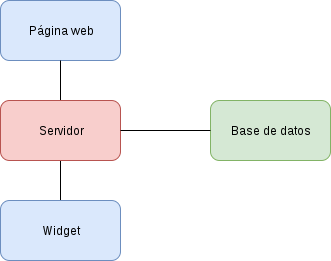
\includegraphics[width=0.5\textwidth]{imgs/descripcion.png}
	\caption{Infraestructura de Colmena}
	\label{infraestructura}
\end{figure}

\subsection{Widget}
El widget es la parte principal del proyecto. Es el objeto que las empresas colocaran en sus tiendas online y que permitirá a los clientes hacer una donación. Consiste en un pequeño rectángulo(\ref{widget}) en el que se le ofrece al a persona que está leyéndolo que aporte una pequeña cantidad de dinero, siempre entre 1 y 5 euros, a un proyecto en concreto. \\

El widget es 100\% personalizable. En la web existe un asistente que permite a las empresas personalizar el widget de modo que este encaje bien en sus comercios online. Este asistente permite cambiar las siguientes características del widget:

\begin{itemize}
	\item \textbf{Proyecto:} Permite elegir a que proyecto destinar el dinero entre los proyectos de Alboan.
	\item \textbf{Opciones de donación:} Permite decidir si la donación será estática, de \EUR{1}, o si esta podrá ser variable, entre 1 y 5 euros.
	\item \textbf{Fondo:} Permite elegir entre una foto, única para cada proyecto, o un fondo de color estático mediante un selector de color.
	\item \textbf{Color de la fuente:} Permite elegir el color de la fuente
\end{itemize}

El widget está compuesto de lenguaje HTML5 y CSS3, no tiene ningún plugin externo, lo que permite incrustarlo en cualquier página web sin que esta se vea afectada o haya que hacer alguna modificación en ella. Se ha desarrollado para que sea responsivo.\\

Por último, la inclusión del widget en la tienda esta simplificada al máximo de manera que la tienda no se vea afectada o tenga que realizar labores de reestructuración del código de su página web. Este proceso se hace mediante un script de código en JavaScript que permite añadir, en el espacio reservado para el mismo, el widget.

\begin{figure}[h]
	\centering
	
\includegraphics[width=1\textwidth]{imgs/widget.png}
	\caption {Widget Colmena}
	\label{widget}
\end{figure}



\subsection{Pagina web}

La página web de la Colmena cubre las labores de publicidad y de soporte del widget. Esta incluye funcionalidades como recoger el certificado de donación después de haber realizado una, crear nuevos widgets para las empresas que quieran añadirlos a su página web o contacto con el soporte de Alboan.\\

La página esta desarrollada en \textit{HTML5}, \textit{CSS3}(mediante el pre procesador \textit{sass}) y \textit{JavaScript}. A parte de estas tecnologías se ha utilizado el framework web \textit{Bootstrap} y una gran cantidad de plugins que permiten una mejor navegabilidad en la página web, entre ellos destaca \textit{JQuery}. Se han seleccionado estas tecnologías tras una investigación sobre las tecnologías más recomendadas para el tipo de proyecto. Dado que no teníamos ningún requerimiento sobre estas, hemos apostado por las tecnologías que más nos apetecía utilizar, innovando en algunas de las situaciones y siendo más conservadores en otras.\\

La página web permite al usuario consultar cierta información y realizar varias opciones. Estas opciones se explican a continuación:

\begin{itemize}
	\item \textbf{Conocer el proyecto Colmena:} Es el comienzo de la página web, tras la introducción, compuesta por una foto, está localizada este apartado. Aquí se explica el funcionamiento y la filosofía del proyecto Colmena.
	\item \textbf{Conocer proyectos de Alboan:} En este apartado se exponen los diferentes proyectos que dispone la ONG Alboan. Los proyectos están expuestos con el nombre de este y el país en el que actúa. Si hacemos clic en cualquiera de los proyectos una ventana se despliega y ofrece más información sobre este.
	\item \textbf{Crear un widget:} En este apartado de la página web se ofrece la posibilidad de crear un widget personalizado. Al hacer clic en el botón que ofrece esta posibilidad se despliega una ventana con un asistente. En este asistente se ofrecen varias opciones para personalizar el widget final. Este asistente no es el definitivo que las empresas usaran para realizar el widget que quieren que sea colocado en su comercio online.
	\item \textbf{Recibir un certificado:} En este apartado los usuarios pueden utilizar el código de donación que reciben al donar en cualquier tienda que tenga implantada la Colmena. Después de introducir los datos en un formulario, se le enviará el certificado de donación al mail que ha especificado.
	\item \textbf{Contactar con el soporte de Colmena:} Este es el último apartado de la página web. En él se puede enviar un mail al soporte de Colmena. Es el método de interlocución entre las empresas que quieran implantar el widget en sus comercios y el soporte de Colmena.
\end{itemize}
\newpage
\subsection{Base de datos}

La base de datos de la Colmena está desarrollada en la base de datos NoSQL por excelencia, MongoDB. Se ha utilizado este tipo de base de datos por la versatilidad que proporciona a la hora de acceder a los datos y al conectarse a ella. Es una base de datos muy ágil por lo que permite consultar en un tiempo muy reducido las donaciones. Por último, se ha utilizado esta base de datos por la experimentación con la misma, al no ser una base de datos SQL el equipo tuvimos las ganas de probarla y ver su potencial.\\

La base de datos se encarga de almacenar todos los datos relativos a las donaciones mediante los siguientes campos:

\begin{itemize}
	\item \textbf{Importe:} El importe de la donación.
	\item \textbf{Usada:} Un booleano que marca si la donación ha sido canjeada por el certificado o no.
	\item \textbf{Fecha:} La fecha dividida por día, mes y año.
	\subitem Día
	\subitem Mes
	\subitem Año
	\item \textbf{idDonacion:} Un id asignado a cada donación.\\
\end{itemize}

Una vez almacenada la donación esta está disponible para canjearla por un certificado de donación en la página web. Una vez el certificado de donación es expedido, los datos de la persona donante se guardan en la base de datos con el fin de hacerle llegar información sobre los proyectos, si así lo desea, o hacer diferentes estadísticas con las que la organización pueda mejorar o cambiar sus métodos. Estos son los datos que se añaden al archivo de la donación:

\begin{itemize}
	\item DNI/CIF: Número de identificación fiscal de la persona física o jurídica.
	\item Nombre y Apellidos: El nombre y los apellidos de la persona física o nombre de la empresa.
	\item Razón social: Denominación por la cual se conoce colectivamente a la empresa y en caso de ser una persona, introducirá la palabra "Individuo"
	\item Correo electrónico
	\item Dirección
	\item Código Postal
	\item Población
	\item Provincia
\end{itemize}


\subsection{Servidor}


El servidor del proyecto es el núcleo del mismo. En el convergen todas las funcionalidades de la solución. Este está desarrollado en Node.js. Tras una investigación de las posibles tecnologías y tras ver que no había requerimientos en este aspecto decidimos utilizar esta herramienta ya que es innovadora y emergente.\\

La funcionalidad que el servidor ofrece a los demás componentes del proyecto se basa en recabar la información necesaria de la base de datos y ofrecérsela a la página web para que esta la utilice en sus funciones. También recaba la información del widget y se lo envía a la base de datos para que esta la almacene. Por último el servidor también se utiliza como sistema de almacenamiento de los widgets para tenerlos centralizados y poder repararlos rápidamente en caso de error.\\

El servidor se desarrolla de esta manera, como pieza central, por el hecho de unificar todas las funcionalidades que el sistema pueda necesitar en el mismo nodo. Gracias a la flexibilidad de Node.js y a los plugins que se ofrecen en \textit{NPM}, el gestor de paquetes para \textit{JavaScript}. Con estos plugins se ha conseguido unificar todas las funcionalidades que sin ellos habría que haber desarrollado mediante otros métodos, por ejemplo, el envío de mails o el sistema de creación del certificado de donación.

\subsection{Visualización}

La visualización de los datos es la parte final del proyecto. Este módulo permite visualizar mediante una serie de gráficos interactivos los datos de las donaciones. Los gráficos, como ya he dicho anteriormente son interactivos para que los usuarios puedan 'jugar' con ellos e ir relacionando los datos. Estos gráficos están divididos en dos:

\begin{itemize}
	\item \textbf{Gráfico de queso:} En este gráfico interactivo los usuarios pueden ir clusterizando la información en diferentes divisiones. La primera división por ejemplo seria la dividir las donaciones por el proyecto al que han donado y posteriormente se podría ir profundizando en más opciones.
	\item \textbf{Gráfico con mapa:} En este gráfico se puede ver un mapa de calor en el que se pueden ver las zonas desde las que más se ha donado.
\end{itemize}

Posteriormente estos gráficos se pueden analizar para sacar conclusiones de ellos y poder ofrecer esta información de vuelta a los donantes y socios de la ONG. Con esta información los donantes pueden ver lo que la entidad está recibiendo y como es la sociedad que les rodea gracias al mapa de calor. Por último, Alboan podrá analizar esta información y tomar algunas decisiones basándose en ella además de añadirla a los informes que publica.


\newpage

\section{Descripción de la realización}
En este apartado se hablará de la metodología que se utilizará para desarrollar el proyecto. En este caso se utilizará SCRUM.\\

\subsection{SCRUM}

Scrum es la metodología que se va a utilizar para desarrollar el proyecto y se define de esta manera:

Scrum es un proceso en el que se aplican de manera regular un conjunto de buenas prácticas para trabajar colaborativamente, en equipo, y obtener el mejor resultado posible de un proyecto. Estas prácticas se apoyan unas a otras y su selección tiene origen en un estudio de la manera de trabajar de equipos altamente productivos.\\

En Scrum se realizan entregas parciales y regulares del producto final, priorizadas por el beneficio que aportan al receptor del proyecto. Por ello, Scrum está especialmente indicado para proyectos en entornos complejos, donde se necesita obtener resultados pronto, donde los requisitos son cambiantes o poco definidos, donde la innovación, la competitividad, la flexibilidad y la productividad son fundamentales.\\

Se va a utilizar esta metodología por las siguientes razones:

\begin{itemize}
	\item El proyecto se espera que sea bastante dinámico por lo que esta metodología ayudará a introducir ciertas modificaciones con relativa sencillez.
	\item Las tecnologías que se van a utilizar en este proyecto no están dominadas por el equipo, por lo que en caso de tener que modificar alguna de ellas con esta metodología será mas sencillo.
	\item Con esta metodología nos será muy fácil crear entregables intermedios.
\end{itemize}

\figura{0.5}{imgs/scrum.png}{Proceso scrum}{scrum}{}

Las iteraciones o sprints será de 3 semanas cada uno. Al comienzo de los sprints se hará una reunión para pensar cuales deben ser las tareas que deben ir dentro de dicho sprint y al final del mismo se realizará la reunión de revisión en la que se revisará el trabajo realizado y las tareas pendientes. Estas reuniones tendrán unos productos intermedios, los cuales serán explicados más adelante.\\



\subsection{Trello}

Trello es una herramienta que sirve para organizar tareas/proyectos en un tablero (boards) al que le podemos asignar el nombre del proyecto que estamos trabajando. Este tablero está compuesto por diferentes listas: 1. “por hacer”, 2. “en proceso” y 3. “finalizada” Trello te hace saber en todo momento la parte del proyecto en que te encuentras.\\


En esta aplicación se irán creando los diferentes paneles para cada sprint. Dentro de cada panel se organizaran las tareas acordadas en la reunión al inicio de cada sprint. En el panel los miembros del equipo se irán asignando las tareas y moviéndolas entre los diferentes estados.

\figura{0.7}{imgs/trello.png}{Tablón Trello}{trello}{}

\subsection{Tareas}
A continuación, se procederá a listar las tareas que tendrá cada uno de los sprints. Estas tareas estarán dividas en los diferentes tablones de Trello para que se asignen a los empleados. El primer sprint mezcla tareas de gestión del proyecto con tareas de desarrollo como la creación de la arquitectura del proyecto, por lo que se puede comenzar el sprint desde el momento en el que se acuerde el proyecto. Esta es la lista de tareas:

\begin{itemize}
	\item T1 - Sprint 1
		\subitem T1.1 - Investigación sobre las tecnologías a utilizar
		\subitem T1.2 - Redactar el documento sobre las tecnologías a utilizar
		\subitem T1.3 - Instalar las herramientas de desarrollo
		\subitem T1.4 - Configurar la herramienta de control de versiones
		\subitem T1.5 - Diseñar la arquitectura del proyecto
	\item T2 - Sprint 2
		\subitem T2.1 - Crear el primer diseño de la página web
		\subitem T2.2 - Crear el primer diseño del widget
		\subitem T2.3 -	Desarrollar la lógica del servidor
		\subitem T2.4 - Pruebas servidor
		\subitem T2.5 - Configurar la base de datos
		\subitem T2.6 - Pruebas base de datos
	\item T3 - Sprint 3
		\subitem T3.1 - Desarrollar la lógica de la página web
		\subitem T3.2 - Desarrollar la lógica del widget
		\subitem T3.3 - Consolidar el diseño de la página web
		\subitem T3.4 - Pruebas de la página web
		\subitem T3.5 - Consolidar el diseño del widget
		\subitem T3.6 - Pruebas del widget
		\subitem T3.7 - Crear manual de usuario para los técnicos de mantenimiento
	\item T4 - Sprint 4
		\subitem T4.1 - Investigar los frameworks de visualización de datos
		\subitem T4.2 - Configurar el frameworks de visualización de datos
		\subitem T4.3 - Pruebas sobre el frameworks de visualización de datos
		\subitem T4.4 - Analizar los datos
		\subitem T4.5 - Extraer las estadísticas de los datos

\end{itemize}


\subsubsection{Investigación sobre las tecnologías a utilizar}
En esta tarea se investigarán las principales tecnologías a utilizar en el proyecto principal. Se buscarán las mejores tecnologías para desarrollar un proyecto web integral. Las principales funciones de las tecnologías serán las siguientes, crear un servidor web, crear una página web, crear un widget responsivo que se comunique con el servidor y crear una base de datos que aloje los datos.

\subsubsection{Redactar el documento sobre las tecnologías a utilizar}
En esta tarea se redactará lo decidido en la tarea anterior. Se explicarán las diferentes tecnologías que se utilizarán y porque se han elegido estas.

\subsubsection{Instalar las herramientas de desarrollo}
En esta tarea se instalarán las herramientas pertinentes para el desarrollo del proyecto y su correspondiente gestión.

\subsubsection{Configurar la herramienta de control de versiones}
En esta tarea se instalará la herramienta seleccionada anteriormente para el control de versiones en online. Ya que en el desarrollo estarán implicadas más de una persona, se utilizará una herramienta de este tipo para controlar más el desarrollo.

\subsubsection{Diseñar la arquitectura del proyecto}
El objetivo de esta tarea será el de crear una arquitectura completa del proyecto que tenga en cuenta todos los elementos de este. Se crearán los diferentes proyectos en las herramientas de programación, con los métodos más generales. También habrá que crear las conexiones entre las diferentes tecnologías.

\subsubsection{Crear el primer diseño de la página web}
En esta tarea se crearán varios mockups para la interfaz de la página web, que luego serán entregados al cliente para que este las revise y decida cual desea.

\subsubsection{Crear el primer diseño del widget}
En esta tarea se crearán varios mockups para la interfaz del widget, que luego serán entregados al cliente para que este las revise y decida cual desea.

\subsubsection{Desarrollar la lógica del servidor}
En esta tarea se desarrollarán todos los métodos y servicios que el servidor tenga que implementar para dar servicio a todos los componentes del proyecto.

\subsubsection{Pruebas servidor}
En esta tarea se deberá probar el servidor ante todo tipo de situaciones para evitar fallos futuros.

\subsubsection{Configurar la base de datos}
En esta tarea se deberá configurar la base de datos para que sea capaz de alojar los datos que el servidor, el widget y la página web.

\subsubsection{Pruebas base de datos}
En esta tarea se deberá probar la base de datos ante todo tipo de situaciones para evitar fallos futuros.

\subsubsection{Desarrollar la lógica de la página web}
En esta tarea se desarrollará el sistema de enrutado y de funcionalidad de la página web.

\subsubsection{Desarrollar la lógica del widget}
En esta tarea se desarrollará la funcionalidad y la conexión con el servidor del widget.

\subsubsection{Consolidar el diseño de la página web}
En esta tarea se establecerá el diseño definitivo de la página web.

\subsubsection{Pruebas de la página web}
En esta tarea se deberá probar la página web ante todo tipo de situaciones para evitar fallos futuros.

\subsubsection{Consolidar el diseño del widget}
En esta tarea se establecerá el diseño definitivo de la página web.

\subsubsection{Pruebas del widget}
En esta tarea se deberá probar el widget ante todo tipo de situaciones para evitar fallos futuros.

\subsubsection{Crear manual de usuario para los técnicos de mantenimiento}
En esta tarea se deberá crear un manual que indique detalladamente como son todos los procesos que hay que realizar para mantener el sistema y crear nuevos widget para las empresas.

\subsubsection{Investigar los frameworks de visualización de datos}
En esta tarea se deberán investigar los frameworks que se utilizarán a posteriori para visualizar los datos extraídos de las donaciones. Los gráficos deberán ser interactivos.

\subsubsection{Configurar el framework de visualización de datos}
En esta tarea se configurará el framework elegido en la tarea anterior.

\subsubsection{Pruebas sobre el framework de visualización de datos}
En esta tarea se deberá probar el framework de visualización de datos ante todo tipo de situaciones para evitar fallos futuros.

\subsubsection{Analizar los datos}
En esta tarea se analizarán los datos extraídos de la base de datos y se cargarán en diagramas para su posterior visualización.

\subsubsection{Extraer las estadísticas de los datos}
En esta tarea se deberán extraer conclusiones de los datos y análisis realizados en la anterior tarea. Se deberá realizar un documento que recoja las conclusiones extraídas del proceso de análisis de los datos.

\section{Productos intermedios}

Gracias a la metodología que se va a utilizar es muy fácil generar productos intermedios. Durante el proceso de desarrollo del proyecto se crearán varios prototipos/mockups del widget y de la página web. Al final de cada sprint se hará una revisión del trabajo que se ha realizado, esto será posible gracias al tablón Trello en el que se podrán ver las tareas realizadas. Para definir los productos intermedios que se van a generar se procede a listarlos a continuación:

\begin{itemize}
	\item Documento sobre el pedido del proyecto
	\item Documento sobre las tecnologías a usar
	\item Documento de seguimiento de las tareas realizadas
	\item Varios prototipos de la página web
	\item Varios prototipos del widget
	\item Manual de usuario para los técnicos que mantendrán el proyecto
	\item Documento de conclusiones sobre las donaciones realizadas
\end{itemize}

Gracias a estos productos intermedios se podrá mantener un seguimiento del proyecto y tener una mejor estimación de las tareas y los tiempos necesarios para estas.
